% =====================================================================
% Deterministic Guardrails and Variance-Aware Evaluation for
% Personalized Multi-Agent Content Generation
%
% Target venue: IEEE Access
%
% COMPILING
%   This compiles as-is with IEEEtran, which ships with every TeX
%   distribution and with Overleaf's default image:
%       pdflatex ieee_access_paper && bibtex ... (references are inline)
%
%   For the official IEEE Access submission, open the "IEEE Access"
%   template on Overleaf and change the line below to
%       \documentclass{ieeeaccess}
%   then move \title/\author into that class's \title{}/\author{} form.
%   Everything from \section{Introduction} onward is unchanged.
%
% BEFORE SUBMITTING - search for "REPLACE" and fix every hit.
% =====================================================================

\documentclass[journal]{IEEEtran}

% IEEE requires Times for body and math. Without this, a compile falls back to
% Computer Modern, which is immediately visible to an editor. newtx is the
% current standard pairing; if a distribution lacks it, "mathptmx" is the
% older equivalent. The official ieeeaccess.cls sets this itself.
% amsmath must load before newtxmath, and amssymb must not load at all:
% newtxmath provides the same symbols and the two clash over \Bbbk.
\usepackage{amsmath}
\usepackage{newtxtext}
\usepackage{newtxmath}

\usepackage{graphicx}
\usepackage{booktabs}
\usepackage{array}
\usepackage{url}
\usepackage[hidelinks]{hyperref}
\usepackage{xcolor}

\graphicspath{{figures/}}

% Flags an unresolved item so it cannot be missed in a proof read.
\newcommand{\REPLACE}[1]{\textcolor{red}{\textbf{[REPLACE: #1]}}}

\begin{document}

% No manual line break: IEEEtran breaks the title itself, and a forced break
% strands a fragment on a line of its own. Kept short enough to set on two
% lines rather than three with an orphaned last word.
\title{Deterministic Guardrails and Variance-Aware Evaluation
for Multi-Agent Content Personalization}

% Author order cannot be changed after publication. Agree it before submitting.
\author{
  Prachi~Sharma,
  Danish~Kaul,
  and~Dishant~Sherawat%
  \thanks{The authors are with the School of Engineering and Technology,
  Sushant University, Gurugram, Haryana, India.}%
  \thanks{Source code, the evaluation dataset and every run report referenced
  in this paper are available from the authors on request.}
}

% The volume/issue header is set by the publisher at production; leaving a
% literal "Vol. XX" in a submitted PDF looks like an unfinished draft.
\markboth{IEEE Access}%
{Gupta: Deterministic Guardrails and Variance-Aware Evaluation}

\maketitle

% ---------------------------------------------------------------- abstract
\begin{abstract}
Large language models (LLMs) generate fluent marketing copy but routinely
fabricate quantitative claims and drift outside the task they were asked to
perform, and the field lacks settled practice for measuring whether an
engineering fix has actually helped. This paper reports a system and a
measurement study. The system is a personalized multi-agent content generator
in which five narrow agents share a three-level user profile, and in which two
interventions are deliberately deterministic rather than model-mediated: a
scope guard that redirects mismatched requests without any model call, and a
grounding guard that flags claim-shaped figures absent from user-supplied data
instead of rewriting them. Adding the guards moves the deterministic suite from
102/105 to 105/108 assertions with the model held fixed; the three residual
failures are then shown, by substituting a larger model and changing nothing
else, to be a capability limit rather than a prompt defect, and the corrected
configuration reaches 110/110. The measurement study then
quantifies how far such results can be trusted. Scoring the same outputs with
an LLM judge three times reveals a mean score spread of 0.51--0.54 on a
five-point scale, and re-running an unchanged configuration moves a per-agent
mean by up to 0.37. Against that noise floor, a seven-model comparison and a
paired A/B test of per-agent model assignment show no significant benefit
(Wilcoxon signed-rank, $n=15$, $p=0.42$, Cohen's $d=-0.12$), contradicting the
intuition that specialized agents merit specialized models. Two defects in the
evaluation apparatus itself were exposed by running it: a rubric whose anchors
silently restricted the judge to three of five scale points across 174 scores,
and a test case whose rubric penalized correct behavior. We argue that
reporting judge variance alongside judge scores should be routine, since
differences smaller than the measured noise are frequently presented as
improvements.
\end{abstract}

\begin{IEEEkeywords}
Large language models, multi-agent systems, content personalization,
LLM-as-a-judge, evaluation methodology, guardrails, hallucination, measurement
reliability.
\end{IEEEkeywords}

% ------------------------------------------------------------ introduction
\section{Introduction}
\IEEEPARstart{L}{arge} language models produce fluent prose across many
domains, yet deploying them for personalized content generation exposes two
problems that fluency does not solve. First, output must conform to a specific
user's brand identity, tone, platform conventions and accumulated preferences,
none of which the model knows. Second, and more consequentially for
professional use, models fabricate specifics. Asked to write marketing copy,
they volunteer percentages, currency amounts and multipliers that no one
supplied, in prose confident enough that a reader has no signal to doubt
it~\cite{ji2023hallucination}.

A natural architecture for the first problem is to decompose the task across
narrow agents, each holding its own instructions and profile, coordinated by a
router~\cite{wu2023autogen, langgraph2024}. A natural approach to the second is
to instruct the model not to invent figures. We implemented both and found the
second does not work: explicit prohibition in the system prompt did not prevent
fabrication, a result consistent with broader findings that prompt-level
constraints are unreliable safety mechanisms~\cite{rebedea2023nemo}.

That observation motivated a design preference that runs through this work.
Where a property can be checked deterministically, we check it in code rather
than asking the model to respect it. Two mechanisms follow. A \emph{scope
guard} compares the evidence a request provides for the selected agent's task
against the evidence for every sibling agent, and redirects the request when
the mismatch is unambiguous --- without a model call, and therefore at no
latency or token cost. A \emph{grounding guard} extracts claim-shaped numeric
patterns from generated copy and checks each against the set of figures the
user actually provided, flagging those it cannot justify.

Having built interventions, we needed to know whether they helped. This is
where the work turned from engineering to measurement. Deterministic assertions
answer narrow questions well --- did the agent hand off, did the budget
allocation sum correctly, did the reply honour a hashtag limit --- but say
nothing about whether copy is any good. The standard remedy is an LLM
judge~\cite{zheng2023judging, liu2023geval}, and judges are known to carry
biases: they favour their own generations~\cite{panickssery2024selfpref},
favour longer answers, and are sensitive to presentation
order~\cite{wang2023fair, koo2023benchmarking}.

What we found is that the practical obstacle is not bias but \emph{variance}.
Scoring identical outputs three times with a fixed judge at temperature zero
produced a mean score spread of 0.51--0.54 on a five-point scale. Re-running an
unchanged system configuration and re-judging moved one agent's mean by 0.37.
Both figures are larger than every per-agent quality difference we were
otherwise preparing to act on. Reported without that context, a 0.3 difference
reads as an improvement; measured against it, the difference is
indistinguishable from noise.

This paper addresses four research questions.

\begin{itemize}
\item \textbf{RQ1.} Do deterministic scope and grounding guards measurably
      improve a personalized multi-agent content system, and which residual
      failures are attributable to model capability rather than system design?
\item \textbf{RQ2.} How reliable is an LLM judge applied to this task, and what
      does its measured variance imply for the differences that may be claimed?
\item \textbf{RQ3.} Among freely available models, how much does the choice of
      generator model affect output quality relative to that variance?
\item \textbf{RQ4.} Does assigning a different model to each specialized agent
      improve quality over a single model serving all of them?
\end{itemize}

Our contributions are:

\begin{enumerate}
\item A personalized multi-agent architecture in which scope enforcement and
      claim grounding are deterministic post-processing stages rather than
      prompt instructions, with measured effect (Section~\ref{sec:rq1}).
\item A reliability protocol for LLM-judge evaluation that reports score spread
      across repeated judgements alongside the scores, together with the
      measured noise floor for this task (Section~\ref{sec:rq2}).
\item A seven-model comparison and a paired A/B test showing that per-agent
      model specialization yields no statistically significant benefit at this
      scale, with the negative result reported in full
      (Sections~\ref{sec:rq3}--\ref{sec:rq4}).
\item Two defects in our own evaluation apparatus, surfaced by executing it: a
      rubric-induced collapse of a five-point scale to three points, and a test
      case whose rubric anchor penalized correct behavior
      (Section~\ref{sec:selfaudit}). We report these because they were more
      instructive than the system results they were meant to produce.
\end{enumerate}

% ----------------------------------------------------------- related work
\section{Related Work}

\subsection{Personalized Text Generation}
Classical personalization relies on explicit user models or collaborative
signals~\cite{koren2009matrix, zhang2020explainable}. For LLMs, three families
dominate. Fine-tuning adapts weights to a user or cohort, which is effective
but costly and impractical per-user. Retrieval-augmented
generation~\cite{lewis2020rag} injects user-specific material at inference,
and the LaMP benchmark~\cite{salemi2023lamp} formalizes personalized generation
as a retrieval-plus-generation task across several sub-problems. Prompt-level
conditioning simply appends profile text, which is cheap and
effective~\cite{brown2020fewshot} but unstructured: profiles tend to accumulate
as free text with no notion of which attributes apply to which task.

Our architecture differs in composing profiles from three nested scopes ---
global, domain and agent --- so an attribute is declared once at the level
where it is true, and an agent receives exactly the union that applies to it.
We are not aware of prior work that reports measured effects for scoped profile
composition in a deployed multi-agent setting, though the mechanism itself is
unsurprising.

\subsection{Multi-Agent LLM Systems}
Agent frameworks such as AutoGen~\cite{wu2023autogen},
CrewAI~\cite{moura2024crewai} and LangGraph~\cite{langgraph2024} coordinate
specialized LLM-powered components built on the transformer
architecture~\cite{vaswani2017attention}, drawing on reasoning-and-acting
patterns~\cite{yao2023react}, intermediate-step
prompting~\cite{wei2022cot}, tool invocation~\cite{schick2023toolformer} and
self-critique~\cite{shinn2023reflexion}. These frameworks principally address
\emph{task decomposition}: splitting a complex objective across cooperating
roles. Comparatively little attention is paid to what happens when a user
addresses the wrong agent, which in a user-facing product is routine rather
than exceptional. Our scope guard targets that case specifically, and we
evaluate it as a first-class mechanism.

\subsection{Hallucination and Guardrails}
Hallucination in generated text is extensively
surveyed~\cite{ji2023hallucination}. Detection approaches include
sampling-based self-consistency checks~\cite{manakul2023selfcheckgpt},
atomic-fact decomposition against references~\cite{min2023factscore}, and
retrieval-grounded metrics~\cite{es2024ragas}. Programmable guardrail systems
such as NeMo Guardrails~\cite{rebedea2023nemo} place a controllable layer
between user and model.

Our grounding guard is narrower than any of these and deliberately so. It does
not assess truth; it assesses \emph{provenance}. A percentage in generated
marketing copy is flagged unless that figure appears in the user's request,
attachment or profile. This is weaker than fact-checking and much cheaper ---
no model call, no retrieval corpus --- and it fits the deployment reality that
only the user knows whether a claim about their product is true. Critically, the
guard flags rather than rewrites: deleting a number mid-sentence yields text
like ``reduce costs by up to,'' which is worse than the original.

\subsection{LLM-as-a-Judge and Its Reliability}
Using a strong model to score generated text is now
standard~\cite{zheng2023judging, liu2023geval}, validated against human
preference at scale~\cite{chiang2024arena}. Known failure modes include
self-preference, where an evaluator rates its own
generations higher~\cite{panickssery2024selfpref}; position and verbosity
effects~\cite{wang2023fair}; and broader cognitive biases documented
systematically by Koo et al.~\cite{koo2023benchmarking}. Mitigations include
swapping presentation order, ensembling multiple judges, and sampling multiple
judgements in the spirit of self-consistency~\cite{wang2023selfconsistency}.

The gap we address is reporting practice rather than method. Judge scores are
commonly published as point estimates, with bias acknowledged qualitatively and
variance not quantified at all. We measure the variance for our task, find it
large enough to subsume the differences we were about to claim, and argue that
an explicit noise floor should accompany any judge-derived comparison. The
observation that LLM evaluation pipelines are themselves under-tested is, to
our knowledge, rarely reported with concrete instances; Section
\ref{sec:selfaudit} supplies two.

% --------------------------------------------------------------- system
\section{System Design}

\subsection{Overview}
The system serves five narrow marketing agents: a social-caption writer, an SEO
optimizer, a campaign planner, and two agents whose deliverable is a rendered
image (a social post image and an ad creative). Each is declared, not coded, as
a specification carrying its instructions, profile field definitions, output
kind and guard configuration; the runtime is shared. A broader earlier
configuration of the same architecture spanned seven domains and 34 agents,
which we use here only to argue that the design is not specific to five agents.

Requests traverse the eight-stage pipeline in Fig.~\ref{fig:pipeline}. Two
stages are highlighted because they are the deterministic interventions this
paper evaluates.

\begin{figure*}[!t]
\centering
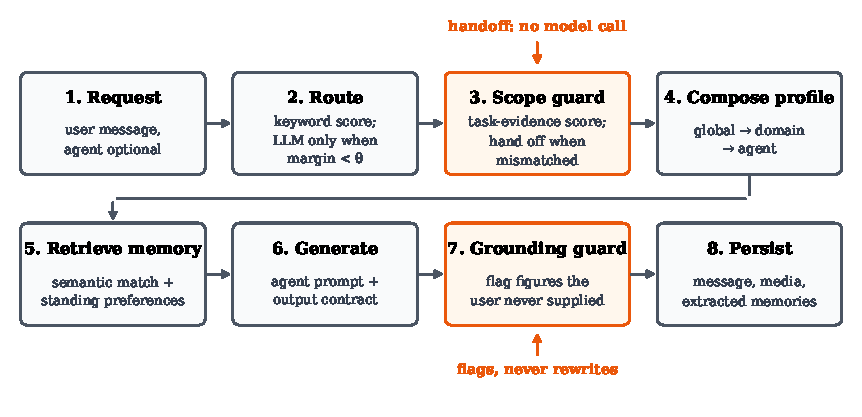
\includegraphics[width=\textwidth]{fig1_pipeline.pdf}
\caption{The request pipeline. Stages 3 and 7 are deterministic: the scope
guard redirects a mismatched request with no model call, and the grounding
guard annotates unsupported figures without altering the generated text.}
\label{fig:pipeline}
\end{figure*}

\subsection{Three-Level Profile Composition}
A user holds a \emph{global} profile (identity, communication style), a
\emph{domain} profile (for marketing: brand name, industry, audience, tone,
palette, prohibited terms) and an \emph{agent} profile (for the caption writer:
platforms, target length, hashtag policy). At request time the three are
composed into a context block, with the narrowest scope taking precedence. A
brand tone is stated once and reaches all five agents; a hashtag policy reaches
only the agent for which it is meaningful.

\subsection{Deterministic Scope Guard}
Let $a$ be the selected agent and $S$ the set of sibling agents. For a request
$r$ we compute a task-evidence score $\tau(x, r)$ for each agent $x$,
accumulating matches of $r$ against the task vocabulary declared by $x$. The
request is redirected to $x^\star = \arg\max_{x \in S} \tau(x, r)$ when all of
the following hold:
\begin{align}
|r| &\ge \lambda_{\min} \label{eq:len}\\
\tau(a, r) &\le \theta_{\text{own}} \label{eq:own}\\
\tau(x^\star, r) &\ge \theta_{\text{other}} \label{eq:other}\\
\tau(x^\star, r) - \tau(a, r) &\ge \delta \label{eq:margin}
\end{align}
with $\lambda_{\min}=15$ characters, $\theta_{\text{own}}=1.5$,
$\theta_{\text{other}}=4.0$ and $\delta=3.0$. The thresholds are deliberately
conservative: a wrong redirect is more damaging to trust than a slightly
off-topic answer, so the guard stays silent unless the mismatch is clear.
Condition~(\ref{eq:len}) suppresses the guard for greetings and
acknowledgements, which carry no task evidence either way.
Condition~(\ref{eq:own}) requires that the selected agent be a genuinely poor
fit rather than merely a worse one, and
conditions~(\ref{eq:other})--(\ref{eq:margin}) require that some sibling be
both strongly indicated and clearly better. All four must hold, so a request
that is ambiguous between two agents is answered by the one the user chose.

One detail proved essential. An early version scored agents using their full
declared vocabulary, including their own \emph{names}. A request such as
``design an ad creative for the free trial'' sent to the caption writer then
scored highly for the caption writer, because the phrase contains words that
appear in its own name, and the request was never redirected. Restricting
$\tau$ to \emph{task} evidence and excluding name matches fixed this. The
router, which selects an agent when the user has not, continues to use the full
score, since there a name match is a legitimate signal of intent.

\subsection{Grounding Guard}
Let $P$ be a set of claim-shaped patterns --- percentages, currency amounts,
bare multipliers such as \texttt{10x}, and ``up to'' constructions --- declared
per agent. Let $N(r, \alpha, \pi)$ be the set of numeric tokens appearing in
the request $r$, any attachment $\alpha$, and the composed profile $\pi$. For
generated text $g$, every match $m \in P$ with numeric token $n(m) \notin
N(r,\alpha,\pi)$ is flagged. The reply is returned unchanged with an appended
notice naming the unsupported figures.

Three refinements were required by observed false positives.
\emph{Cadence expressions} such as ``3x per week'' are schedules, not claims,
and are excluded by a negative lookahead over temporal units.
\emph{Self-labelled proposals} such as ``20\% (suggested figure)'' are
explicitly marked as proposals --- behavior the campaign planner's instructions
request --- and flagging them penalized compliance.
\emph{Budget allocation} is legitimate for the planner: given a user-supplied
total $T$, currency amounts $\le T$ are permitted, enabled per agent so the
exemption does not leak to agents that have no business allocating money.

The guard reads text only. When a user attaches an image, a figure the model
read off that image is indistinguishable from one it invented, so the notice
changes wording to say the check cannot see images rather than asserting
fabrication.

% ------------------------------------------------------------ methodology
\section{Evaluation Methodology}

\subsection{Dataset}
The dataset is 30 request cases held as declarative data, spanning twelve
categories (Table~\ref{tab:dataset}). Categories were chosen to cover the
failure modes we cared about rather than to sample naturally occurring traffic
--- a limitation we return to in Section~\ref{sec:threats}. Five cases are
marked as requiring a real model and are skipped under the deterministic
composer, because that composer ignores agent instructions by construction and
running them would say nothing about prompt quality.

\begin{table}[!t]
\caption{Evaluation dataset composition (30 cases)}
\label{tab:dataset}
\centering
\footnotesize
\begin{tabular}{@{}lr@{\hspace{2em}}lr@{}}
\toprule
Category & $n$ & Category & $n$\\
\midrule
ordinary        & 7 & grounding      & 4\\
out of scope    & 6 & complex        & 3\\
profile         & 2 & routing        & 2\\
ambiguous       & 1 & attachment     & 1\\
brand           & 1 & clarification  & 1\\
memory          & 1 & platform       & 1\\
\bottomrule
\end{tabular}
\end{table}

\subsection{Deterministic Assertions}
Each case declares machine-checkable assertions: expected output kind, whether
a scope handoff should occur and to which agent, rendered media dimensions,
substrings that must or must not appear, hashtag and length limits, whether
profile content reached the assembled prompt, and whether a stored memory was
retrieved. A run yields 110 assertions over the 30 cases. Every run records the
provider, model, temperature, token budget, embedding configuration and guard
thresholds, and the comparison tool refuses to compare runs that differ in
these respects.

\subsection{Rubric and Judge}
Qualitative dimensions are defined in a human-readable rubric of 32 dimensions
across five groups, each with anchors at levels 1, 3 and 5. A case declares
which dimensions apply to it; 22 of the 30 cases are scorable, the remaining
eight being scope handoffs and routing decisions that produce no creative
output.

The judge receives the brand context the run actually configured, the request,
the output, and the anchors for that case's dimensions, and returns a score and
a one-sentence justification per dimension at temperature zero. Two dimensions
--- \texttt{legibility} and \texttt{brand\_fit} --- are properties of rendered
pixels; since the judge receives only the image specification and alt text,
these are reported as unjudged rather than guessed. Layout legibility is
instead checked deterministically across 27 size-and-payload combinations.

The rubric is parsed from the same prose document a human reader uses, so the
machine-readable and human-readable versions cannot diverge. A consistency
check asserts in both directions that every dimension a case declares exists in
the rubric and every dimension defined is used by some case.

\subsection{Reliability Protocol}
\label{sec:protocol}
The protocol below is what Section~\ref{sec:rq2} quantifies, and what every
comparison in Section~\ref{sec:rq4} depends on.

The judge scores each case $N$ times. We report the \emph{median} as the score
and the \emph{spread} (maximum minus minimum) as the uncertainty. With $N=1$ no
spread is reported, since unknown is not the same as zero. Runs are comparable
only when judge model, judge prompt version, rubric file and $N$ all match; the
comparison tool enforces this. When the judge model equals the model that
produced the output, the condition is flagged in the terminal, the stored
results and the rendered report, because self-preference makes such a figure an
upper bound rather than a measurement~\cite{panickssery2024selfpref}.

\subsection{Reproducibility}
All reported numbers derive from stored run artefacts rather than from
transcription: every figure in this paper is generated by a script that reads
those artefacts, so a figure cannot drift from the result it depicts. Hardware
was a 4-core Intel i5-10210U without GPU. Local models ran under Ollama;
hosted models were reached through an OpenAI-compatible endpoint.

% ---------------------------------------------------------------- results
\section{Results}

\subsection{RQ1: Effect of the Deterministic Guards}
\label{sec:rq1}
Table~\ref{tab:rq1} reports the deterministic suite before and after the
guards, holding the model and all settings fixed at a local 3B model.

\begin{table}[!t]
\caption{Deterministic suite, before and after the guards (identical model and settings)}
\label{tab:rq1}
\centering
\footnotesize
\begin{tabular}{@{}lcc@{}}
\toprule
 & Baseline & With guards\\
\midrule
Assertions passed            & 102/105 & \textbf{105/108}\\
Errors                       & 0 & 0\\
Degraded image specifications& 0 & 0\\
``write ad copy'' routes to  & ad-creative (image) & \textbf{social-copy}\\
Supplied \$400 budget        & not asserted & \textbf{sums to \$400}\\
Invented figures             & undetected & \textbf{flagged}\\
Elapsed (21 generating cases)& 1215\,s & 1322\,s\\
\bottomrule
\end{tabular}
\end{table}

The guards added three assertions and passed them. The 9\% latency increase is
the cost of longer instructions; no prompt change made the system faster and
none was claimed to.

Three failures persisted, all on cases requiring the model to ask a clarifying
question or to refrain from inventing figures. No prompt revision moved them.
Substituting a larger hosted model, with every other setting unchanged, closed
all three and reduced elapsed time from 1325\,s to 88\,s. We therefore
attribute those residual failures to model capability rather than system
design --- a distinction that deterministic assertions alone cannot draw, and
that only a controlled model substitution could establish.

That substitution also exposed two false positives in our own grounding guard
that the weaker model had never triggered, because it never produced the
constructions involved: a posting cadence and a self-labelled proposal, both
described in Section~III-D. Both were corrected, and the corrected guard is
checked in both directions --- unlabelled claims are still caught.

\subsection{RQ2: Judge Reliability and a Rubric-Induced Scale Collapse}
\label{sec:rq2}

Judging the full suite with an independent model (not the generator) produced a
mean of 4.23/5 across 61 dimension scores. Taken alone this number is close to
meaningless, which is the point of this subsection.

First, the scale. Across 174 individual judgements under our initial judge
prompt, \emph{every score was 1, 3 or 5}; levels 2 and 4 were never used
(Fig.~\ref{fig:collapse}). The cause was the rubric: its tables define anchors
at 1, 3 and 5, and the judge treated those as the only admissible answers. A
five-point instrument had silently become a three-point one. Naming the
intermediate levels explicitly in the prompt restored them --- 10.4\% of
subsequent scores were even-valued --- and reduced the worst observed spread
from 4 to 2.

\begin{figure}[!t]
\centering
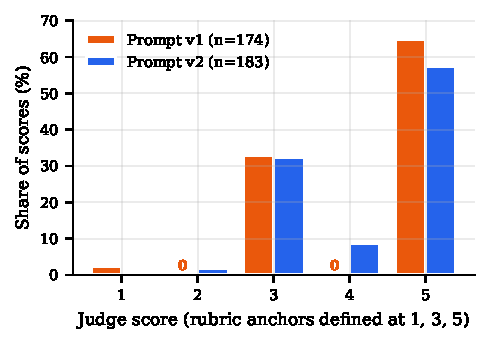
\includegraphics[width=\columnwidth]{fig2_scale_collapse.pdf}
\caption{Judge score distribution before and after the judge prompt named the
intermediate scale levels. Under v1 no score of 2 or 4 occurred in 174
judgements, because the rubric defines anchors only at 1, 3 and 5.}
\label{fig:collapse}
\end{figure}

Second, the variance. Scoring identical outputs three times at temperature zero
gave 62--69\% exact agreement, a mean spread of 0.51--0.54 and a worst-case
spread of 4 on a five-point scale. Re-running an unchanged configuration and
re-judging moved one agent's mean by 0.37 with no change to the system at all.
We adopt 0.5 as the noise floor for this task: differences below it are not
results. An earlier screening pass used 0.33 and duly identified two per-agent
``winners'' that Section~\ref{sec:rq4} shows to be spurious.

Scores are therefore comparable only within a fixed judge model, prompt version
and repeat count, all of which we record with every stored result.

\subsection{RQ3: How Much Does the Generator Model Matter?}
\label{sec:rq3}

We evaluated every model available to us at no cost --- seven of twenty-two
offered by the hosted provider; the remainder required paid credits --- holding
the dataset, thresholds and judge fixed and changing only the generator
(Table~\ref{tab:bakeoff}, Fig.~\ref{fig:bakeoff}).

\begin{table}[!t]
\caption{Seven-model comparison. Same dataset, thresholds and judge; only the generator model differs}
\label{tab:bakeoff}
\centering
\footnotesize
\begin{tabular}{@{}lccrc@{}}
\toprule
Model & Judge & Assertions & Time (s) & Errors\\
\midrule
beam                 & 4.16 & 108/110 & 142 & 0\\
gemma4:31b           & 4.15 & 109/110 & \textbf{43} & 0\\
gpt-oss:20b          & 3.89 & 105/110 & 113 & 0\\
nemotron-3-ultra     & 3.87 & 107/110 & 386 & 0\\
nemotron-3-super     & 3.80 & 107/110 & 731 & 0\\
gpt-oss:120b$^{a}$   & 3.52 & 103/110 & 83  & 0\\
nemotron-3-nano:30b$^{b}$ & --- & 80/82 & 563 & 9\\
\bottomrule
\multicolumn{5}{@{}l@{}}{\footnotesize $^{a}$Judged itself; score is an upper bound.}\\
\multicolumn{5}{@{}l@{}}{\footnotesize $^{b}$Excluded: 9 of 30 cases errored, so its}\\
\multicolumn{5}{@{}l@{}}{\footnotesize \phantom{$^{b}$}mean describes an easier subset.}\\
\end{tabular}
\end{table}

\begin{figure}[!t]
\centering
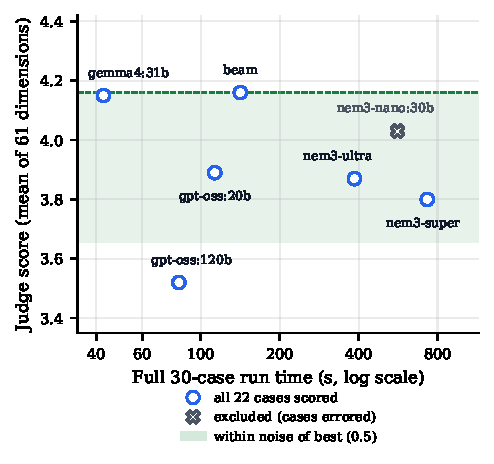
\includegraphics[width=\columnwidth]{fig3_bakeoff.pdf}
\caption{Judge score against wall-clock run time for every freely available
model. Five of six comparable models fall within the measured noise floor of
the best, while run time varies by a factor of seventeen.}
\label{fig:bakeoff}
\end{figure}

The leading two models differ by 0.01, far inside the noise floor, while
differing by a factor of 3.3 in run time. Five of the six comparable models lie
within 0.5 of the best. The practical conclusion is that for this task,
selection among freely available models should be driven by latency and
reliability, which are measured precisely, rather than by judge score, which is
not.

Two incidental findings deserve note. The largest model tested scored
\emph{lowest} despite judging its own output, a condition that should have
inflated it. And one model could not complete the suite at all, for a reason
that turned out to be a defect in our own client (Section~\ref{sec:reasoning}).

\subsection{RQ4: Per-Agent Model Specialization}
\label{sec:rq4}

A multi-agent architecture invites the hypothesis that each specialized agent
should use the model best suited to it. The screening pass in
Section~\ref{sec:rq3} appeared to support this, identifying two agents whose
scores improved by 0.45 and 0.33 under non-default models.

We tested the hypothesis directly. A mixed-fleet configuration pinned those two
agents to their apparent best models; a control arm used one model throughout.
Both arms were freshly generated and judged under the protocol of
Section~\ref{sec:protocol} with three repeats (Fig.~\ref{fig:ab},
Table~\ref{tab:ab}).

\begin{table}[!t]
\caption{Paired A/B: one model for all agents versus a mixed fleet}
\label{tab:ab}
\centering
\footnotesize
\begin{tabular}{@{}lcc@{}}
\toprule
 & One model & Mixed fleet\\
\midrule
Overall judge mean        & \textbf{4.28} & 4.18\\
Assertions               & 109/110 & 109/110\\
Elapsed                  & \textbf{54\,s} & 201\,s\\
ad-creative (pinned)     & \textbf{4.56} & 4.33\\
social-copy (pinned)     & 3.80 & \textbf{3.87}\\
post-image (unchanged)   & \textbf{4.25} & 3.88\\
\bottomrule
\end{tabular}
\end{table}

\begin{figure}[!t]
\centering
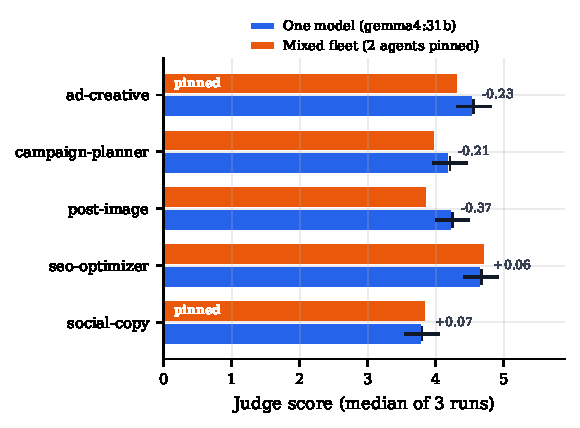
\includegraphics[width=\columnwidth]{fig4_ab_per_agent.pdf}
\caption{Per-agent scores for both arms. Whiskers show the judge's own mean
spread on the control arm. Every between-arm gap, including for the two pinned
agents, lies inside that spread.}
\label{fig:ab}
\end{figure}

Of 61 paired dimension scores, 46 were unchanged. Among the 15 that moved, 7
favoured the mixed fleet and 8 the single model. A Wilcoxon signed-rank
test~\cite{wilcoxon1945} on the paired scores gives $W = 45.5$, $n = 15$,
$p = 0.42$ (exact, two-sided), with Cohen's $d = -0.12$: no significant
difference, negligible effect size. We use a signed-rank test rather than a
paired $t$-test because the scores are ordinal and discrete, and the exact
distribution is tractable at this $n$. The mixed fleet was nonetheless 3.7
times slower.

The decisive observation is the third row of Fig.~\ref{fig:ab}. The
\texttt{post-image} agent used the \emph{same} model in both arms and its mean
still moved by 0.37. Generation at non-zero temperature plus judge
disagreement produces per-agent movement of that magnitude with no
configuration change whatsoever. The screening gaps of 0.33 and 0.45 were
within that band, and did not survive confirmation; one of the two pinned
agents got measurably \emph{worse}.

We therefore reject the per-agent specialization hypothesis at this scale. We
emphasise that this is a negative result about effect size relative to noise,
not evidence that model choice never matters; a task with wider genuine quality
separation could well reach the opposite conclusion.

\subsection{Self-Audit: Defects in the Evaluation Apparatus}
\label{sec:selfaudit}

Two defects in the evaluation were found by running it, and both would have
silently corrupted conclusions.

The \emph{scale collapse} of Section~\ref{sec:rq2} is the first. A rubric that
reads correctly to a human restricted the judge to three of five levels across
174 judgements. Nothing in the pipeline would have surfaced this; it was
visible only on inspecting the score distribution, which we had no particular
reason to plot.

The second was a \emph{self-contradictory test case}. A case intended to test
profile awareness configured the agent's content type as ``landing page'' while
the request asked for ``a blog post.'' The agent followed the explicit request
and stated that it had done so, which is the correct precedence. The rubric
anchor for that dimension rewarded adherence to the configured profile, and so
scored correct behavior 1/5 --- unanimously across three repeats. The defect
lay in the rubric and the case, not the system. We corrected the anchor to state
that an explicit request overrides a standing default, removed the
contradiction from the case, and added a companion case that deliberately
exercises the override.

Both incidents share a shape: the apparatus was internally consistent and
externally wrong, and the error presented as a confident number. We draw the
methodological conclusion in Section~\ref{sec:discussion}.

\subsection{A Client Defect Masquerading as Provider Failure}
\label{sec:reasoning}

During RQ3, four of six models failed between 4 and 19 of 30 cases with what
appeared to be provider outages. The cause was neither the provider nor the
models. Models that spend completion tokens on hidden reasoning before
answering can exhaust the token budget mid-thought, in which case the API
returns HTTP 200 with an empty message body and a finish reason of
\texttt{length}. Our client treated an empty body as a provider failure. On one
model, 1 request in 6 returned 700 completion tokens and zero characters of
content.

Treating that specific signature --- empty content with a length finish reason,
or a populated reasoning field with no answer --- as a budget condition and
retrying once with threefold headroom reduced five of six models to zero
errors. The sixth remains unusable for this task: it produced 12{,}000 to
16{,}000 characters of reasoning and no answer even at a 4{,}000-token ceiling,
requiring 41 retries in a single run.

We report this because it affected comparability rather than merely robustness.
Before the fix, each model errored on a different number of cases, so each
model's score described a different subset of the dataset. Any ranking computed
across those runs would have been an artefact of which cases happened to
survive.

\subsection{Latency and Cost}
Table~\ref{tab:perf} contrasts a local 3B model on commodity hardware with a
hosted 31B model. On CPU, prompt evaluation dominates, so latency tracks prompt
size as much as reply length.

\begin{table}[!t]
\caption{Latency and cost. Hardware: 4-core Intel i5-10210U, no GPU}
\label{tab:perf}
\centering
\footnotesize
\begin{tabular}{@{}lcc@{}}
\toprule
Operation & Local 3B & Hosted 31B\\
\midrule
Text agent                & 28--53\,s & 1.3--3.2\,s\\
Image agent (spec + render)& 28--64\,s & 1.4--2.4\,s\\
Scope handoff             & $<$1\,ms & $<$1\,ms\\
Full 30-case run          & 1325\,s & 49--88\,s\\
Cost per run              & --- & \$0.0039\\
\bottomrule
\end{tabular}
\end{table}

The scope handoff requires no model call, so a redirected request costs no
tokens and returns effectively instantly regardless of backend --- the clearest
practical argument for implementing that check deterministically.

% ------------------------------------------------------------- discussion
\section{Discussion}
\label{sec:discussion}

\textbf{Prompt instructions are not a safety mechanism.} Explicit prohibition
did not stop figure fabrication; a deterministic post-processing check did. This
agrees with the premise behind programmable guardrail
systems~\cite{rebedea2023nemo} and suggests a simple design heuristic: if a
property can be checked in code, check it in code, and reserve the model for
what only a model can do.

\textbf{Flagging beats rewriting for provenance.} An automatic rewrite that
removes an unsupported figure damages the sentence containing it, and the system
cannot know whether the claim was true --- only the user can. Annotating
preserves both the text and the user's authority over it.

\textbf{Report the noise floor, not just the score.} This is our main
methodological claim. Our judge disagreed with itself by roughly half a point
on a five-point scale, and total run-to-run movement reached 0.37 on an
unchanged configuration. Differences of 0.3 are routinely presented as
improvements in informal practice. Publishing a judge score without its
variance invites exactly the error we made during screening and caught only by
confirming. A noise floor is cheap to obtain --- re-judge $N$ times and report
the spread --- and changes which conclusions are available.

\textbf{Architectural specialization does not imply model specialization.} The
appeal of giving each narrow agent its own model is strong and, at this scale,
unsupported: no significant difference, negligible effect size, 3.7 times the
latency, and more operational complexity. One model served five agents as well
as five models did.

\textbf{Evaluation code deserves the same scrutiny as system code.} Both
defects in Section~\ref{sec:selfaudit} were in the measuring apparatus, and both
produced plausible numbers. We found them only because we plotted a
distribution and re-read a low score we did not believe. Meta-evaluation ---
testing the evaluator --- is not a formality.

\subsection{Implications for Practitioners}
Four of our findings translate directly into deployment practice, and we state
them separately because each is cheap to adopt.

First, separate the two kinds of check. Deterministic assertions over
machine-verifiable properties are fast, free and stable, and they should carry
as much of the evaluation burden as possible; reserve judge scoring for
properties that genuinely require reading. In our suite, 110 assertions cover
routing, handoff, provenance, geometry, length and profile propagation, leaving
32 rubric dimensions for the judge.

Second, record the configuration with the result. Every stored run in this work
carries its provider, model, temperature, token budget, embedding settings,
guard thresholds and, after the defect in Section~\ref{sec:reasoning}, its
per-agent model assignments. The comparison tool refuses to compare runs that
differ in any of these. This sounds bureaucratic until a mixed-model run is
indistinguishable from a single-model run in the archive, which was briefly the
case here.

Third, make the evaluator's uncertainty a first-class output. Reporting a
median with its spread costs one extra field and $N$ times the judge calls ---
in our case 213\,s and no monetary cost --- and it is the difference between a
conclusion and a guess.

Fourth, prefer flagging to silent correction wherever the system cannot verify
the property itself. The grounding guard annotates; the scope guard redirects
and says why; the empty-reply handler retries and then reports the specific
cause. In each case the user retains the information needed to override the
system, which matters more in content generation than a marginally cleaner
output would.

% --------------------------------------------------------------- threats
\section{Threats to Validity}
\label{sec:threats}

\textbf{Construct validity.} Judge scores are a proxy for human judgement, not
a measurement of quality. We did not conduct a human scoring pass, so we cannot
report agreement between our judge and human raters; this is the most important
limitation of the work. Self-preference was controlled by using a judge
different from the generator in all reported comparisons and by flagging the
one case where it was not, but verbosity and leniency effects were not
controlled: 36 of 61 median scores were 5s.

\textbf{Internal validity.} Agents generate at temperature 0.4, so arms differ
in generated text as well as configuration; our A/B therefore measures the
combined effect and we report the control arm's own variance to bound it. The
Wilcoxon test rests on 15 non-tied pairs, which is small, and a larger dataset
could detect effects we cannot. Two of the scored dimensions were excluded as
unjudgeable from text, so image agents are scored on fewer dimensions than
text agents.

\textbf{External validity.} All results use a single synthetic brand in one
industry, one language, and one set of five agents. The 30 cases were authored
to probe failure modes we anticipated, not sampled from production traffic, so
category proportions do not reflect real usage. The free-model set is specific
to one provider at one point in time, and model availability changes. The noise
floor of 0.5 is a property of this task and judge, not a constant.

\textbf{Conclusion validity.} RQ4 reports a negative result; absence of a
significant difference at $n=15$ is not evidence of absence of any effect. Our
claim is bounded accordingly: per-agent specialization is unjustified
\emph{at this scale and for this task}, because any true effect is smaller than
the variance we measured.

% ------------------------------------------------------------ conclusion
\section{Conclusion}

We presented a personalized multi-agent content generation system in which
scope enforcement and claim grounding are deterministic rather than
prompt-mediated, and a measurement study of what can honestly be concluded
about such a system. The guards took the deterministic suite from 102/105 to
110/110, and a controlled model substitution showed the residual failures to be
a capability limit rather than a design defect.

The measurement results are the more transferable contribution. An LLM judge
applied to this task disagreed with itself by a mean spread of 0.51--0.54 on a
five-point scale, and an unchanged configuration moved a per-agent mean by
0.37. Against that floor, neither the seven-model comparison nor a paired A/B
of per-agent model assignment showed a significant benefit
($p = 0.42$, $d = -0.12$), and the mixed fleet cost 3.7 times the latency.
Running the evaluation also surfaced two defects in the evaluation itself, each
of which had been producing confident and wrong numbers.

We conclude that judge-derived comparisons should be published with a measured
noise floor, that evaluation apparatus warrants the same testing discipline as
the system under test, and that architectural specialization should not be
assumed to justify model specialization without a paired, repeated measurement.

Future work should establish human--judge agreement for this task, extend the
dataset beyond a single brand and language, and test whether the noise floor we
measured is characteristic of marketing-copy evaluation or of our judge in
particular.

% ------------------------------------------------------------ references
\begin{thebibliography}{99}
\bibitem{brown2020fewshot}
T.~B. Brown \emph{et al.}, ``Language models are few-shot learners,'' in
\emph{Advances in Neural Information Processing Systems}, vol.~33, 2020,
pp.~1877--1901.

\bibitem{vaswani2017attention}
A.~Vaswani \emph{et al.}, ``Attention is all you need,'' in \emph{Advances in
Neural Information Processing Systems}, vol.~30, 2017.

\bibitem{wu2023autogen}
Q.~Wu \emph{et al.}, ``AutoGen: Enabling next-gen LLM applications via
multi-agent conversation,'' arXiv:2308.08155, 2023.

\bibitem{moura2024crewai}
J.~Moura, ``CrewAI: Framework for orchestrating role-playing autonomous AI
agents,'' GitHub repository, 2024. [Online]. Available:
\url{https://github.com/crewAIInc/crewAI}

\bibitem{langgraph2024}
LangChain, ``LangGraph: Build resilient language agents as graphs,''
documentation, 2024. [Online]. Available:
\url{https://langchain-ai.github.io/langgraph/}

\bibitem{yao2023react}
S.~Yao \emph{et al.}, ``ReAct: Synergizing reasoning and acting in language
models,'' in \emph{Proc. Int. Conf. Learning Representations (ICLR)}, 2023.

\bibitem{schick2023toolformer}
T.~Schick \emph{et al.}, ``Toolformer: Language models can teach themselves to
use tools,'' in \emph{Advances in Neural Information Processing Systems},
vol.~36, 2023.

\bibitem{shinn2023reflexion}
N.~Shinn \emph{et al.}, ``Reflexion: Language agents with verbal reinforcement
learning,'' in \emph{Advances in Neural Information Processing Systems},
vol.~36, 2023.

\bibitem{wei2022cot}
J.~Wei \emph{et al.}, ``Chain-of-thought prompting elicits reasoning in large
language models,'' in \emph{Advances in Neural Information Processing Systems},
vol.~35, 2022.

\bibitem{wang2023selfconsistency}
X.~Wang \emph{et al.}, ``Self-consistency improves chain of thought reasoning
in language models,'' in \emph{Proc. Int. Conf. Learning Representations
(ICLR)}, 2023.

\bibitem{koren2009matrix}
Y.~Koren, R.~Bell, and C.~Volinsky, ``Matrix factorization techniques for
recommender systems,'' \emph{Computer}, vol.~42, no.~8, pp.~30--37, 2009.

\bibitem{zhang2020explainable}
Y.~Zhang and X.~Chen, ``Explainable recommendation: A survey and new
perspectives,'' \emph{Foundations and Trends in Information Retrieval},
vol.~14, no.~1, pp.~1--101, 2020.

\bibitem{lewis2020rag}
P.~Lewis \emph{et al.}, ``Retrieval-augmented generation for
knowledge-intensive NLP tasks,'' in \emph{Advances in Neural Information
Processing Systems}, vol.~33, 2020, pp.~9459--9474.

\bibitem{salemi2023lamp}
A.~Salemi, S.~Mysore, M.~Bendersky, and H.~Zamani, ``LaMP: When large language
models meet personalization,'' arXiv:2304.11406, 2023.

\bibitem{ji2023hallucination}
Z.~Ji \emph{et al.}, ``Survey of hallucination in natural language
generation,'' \emph{ACM Computing Surveys}, vol.~55, no.~12, pp.~1--38, 2023.

\bibitem{manakul2023selfcheckgpt}
P.~Manakul, A.~Liusie, and M.~J.~F. Gales, ``SelfCheckGPT: Zero-resource
black-box hallucination detection for generative large language models,'' in
\emph{Proc. Conf. Empirical Methods in Natural Language Processing (EMNLP)},
2023.

\bibitem{min2023factscore}
S.~Min \emph{et al.}, ``FActScore: Fine-grained atomic evaluation of factual
precision in long form text generation,'' in \emph{Proc. Conf. Empirical
Methods in Natural Language Processing (EMNLP)}, 2023.

\bibitem{es2024ragas}
S.~Es, J.~James, L.~Espinosa-Anke, and S.~Schockaert, ``RAGAS: Automated
evaluation of retrieval augmented generation,'' in \emph{Proc. Conf. European
Chapter of the ACL (EACL): System Demonstrations}, 2024.

\bibitem{rebedea2023nemo}
T.~Rebedea, R.~Dinu, M.~Sreedhar, C.~Parisien, and J.~Cohen, ``NeMo Guardrails:
A toolkit for controllable and safe LLM applications with programmable rails,''
in \emph{Proc. Conf. Empirical Methods in Natural Language Processing (EMNLP):
System Demonstrations}, 2023.

\bibitem{zheng2023judging}
L.~Zheng \emph{et al.}, ``Judging LLM-as-a-judge with MT-Bench and Chatbot
Arena,'' in \emph{Advances in Neural Information Processing Systems}, vol.~36,
2023.

\bibitem{liu2023geval}
Y.~Liu \emph{et al.}, ``G-Eval: NLG evaluation using GPT-4 with better human
alignment,'' in \emph{Proc. Conf. Empirical Methods in Natural Language
Processing (EMNLP)}, 2023.

\bibitem{panickssery2024selfpref}
A.~Panickssery, S.~R. Bowman, and S.~Feng, ``LLM evaluators recognize and favor
their own generations,'' arXiv:2404.13076, 2024.

\bibitem{wang2023fair}
P.~Wang \emph{et al.}, ``Large language models are not fair evaluators,''
arXiv:2305.17926, 2023.

\bibitem{koo2023benchmarking}
R.~Koo \emph{et al.}, ``Benchmarking cognitive biases in large language models
as evaluators,'' arXiv:2309.17012, 2023.

\bibitem{chiang2024arena}
W.-L. Chiang \emph{et al.}, ``Chatbot Arena: An open platform for evaluating
LLMs by human preference,'' in \emph{Proc. Int. Conf. Machine Learning (ICML)},
2024.

\bibitem{wilcoxon1945}
F.~Wilcoxon, ``Individual comparisons by ranking methods,'' \emph{Biometrics
Bulletin}, vol.~1, no.~6, pp.~80--83, 1945.
\end{thebibliography}

% IEEE Access requires an author biography. Swap to \IEEEbiography and supply
% a photograph if you have one that meets the template's size requirements;
% IEEEbiographynophoto is acceptable and is used here.
\begin{IEEEbiographynophoto}{Prachi Sharma}
is with the School of Engineering and Technology, Sushant University, Gurugram,
Haryana, India. Their research interests include applied large language model systems,
 multi-agent architectures and the evaluation of generative systems.
\end{IEEEbiographynophoto}

\begin{IEEEbiographynophoto}{Danish Kaul}
is with the School of Engineering and Technology, Sushant University, Gurugram,
Haryana, India. Their research interests include applied large language model systems,
 multi-agent architectures and the evaluation of generative systems.
\end{IEEEbiographynophoto}

\begin{IEEEbiographynophoto}{Dishant Sherawat}
is with the School of Engineering and Technology, Sushant University, Gurugram,
Haryana, India. Their research interests include applied large language model systems,
 multi-agent architectures and the evaluation of generative systems.
\end{IEEEbiographynophoto}

\end{document}
